\chapter{Deep Kalman Filters}\label{chap:dkf}

\section{Introduction}

The Deep Kalman Filter (DKF) keeps the structure of the Kalman filter but
uses neural networks for the state transition, the observation model and
the inference. The linear-Gaussian equations \eqref{eq:1} and
\eqref{eq:2} are replaced by
\begin{equation}
    \mathbf{z}_t \sim \mathcal{N}\big(\mathbf{G}_{\alpha}(\mathbf{z}_{t-1},
    \mathbf{u}_t, \Delta_{t}),\ \mathbf{S}_{\beta}(\mathbf{z}_{t-1},
    \mathbf{u}_t, \Delta_{t})\big)
    \label{eq:3}
\end{equation}
and
\begin{equation}
    \mathbf{x}_t \sim \mathbf{\Pi}\big(\mathbf{F}_{\kappa}(\mathbf{z}_{t})
    \big),
    \label{eq:4}
\end{equation}
where $\mathbf{G}_{\alpha}$, $\mathbf{S}_{\beta}$ and
$\mathbf{F}_{\kappa}$ are neural networks, $\Delta_t$ is the time elapsed
since the previous observation, and $\mathbf{\Pi}$ is a distribution
(Gaussian, Bernoulli, \ldots) whose parameters are output by
$\mathbf{F}_{\kappa}$.

As for a VAE, Krishnan et al.\ \cite{krishnan2015deep} use variational
inference to learn the model
$p_{\theta}(\mathbf{x}_{1:T}, \mathbf{z}_{1:T} \mid \mathbf{u}_{1:T})$.
Two things differ from a standard VAE: there is a sequence of inputs
$\mathbf{u}_{1:T}$, and the latent variables
$\mathbf{z}_{1:T} = \{\mathbf{z}_{t}\}_{t=1}^{T}$ are linked over time,
so the observations $\mathbf{x}_{1:T}$ are not independent either.

\begin{story}[Conditioning on known inputs]
The inputs $\mathbf{u}_{1:T}$ are known and need not be random:
conditioning on them simply means that the model is a family of
distributions over $(\mathbf{x}, \mathbf{z})$ indexed by $\mathbf{u}$. In
a graphical model, such inputs can be drawn as nodes that are always
observed, and d-separation applies unchanged.
\end{story}

\section{Model Specification}

\paragraph{Latent dynamics.}
\begin{align*}
    \mathbf{z}_t \sim&\ \mathcal{N}\big(\mathbf{G}_{\alpha}
    (\mathbf{z}_{t-1}, \mathbf{u}_t, \Delta_{t}),\
    \mathbf{S}_{\beta}(\mathbf{z}_{t-1}, \mathbf{u}_t, \Delta_{t})\big),
    \qquad t \geq 1,
\end{align*}
with $\mathbf{S}_{\beta}$ a diagonal covariance matrix. For $t = 1$ the
\enquote{previous state} is an initial value $\mathbf{z}_{0}$, which in my
implementation is either fixed at $\mathbf{0}$ or a learned parameter.

\paragraph{Observation model.}
\[
    \mathbf{x}_t \sim p(\mathbf{x}_t \mid \mathbf{z}_{t}) =
    \mathbf{\Pi}\big(\mathbf{F}_{\kappa}(\mathbf{z}_{t})\big).
\]

\begin{figure}[ht!]
    \centering
    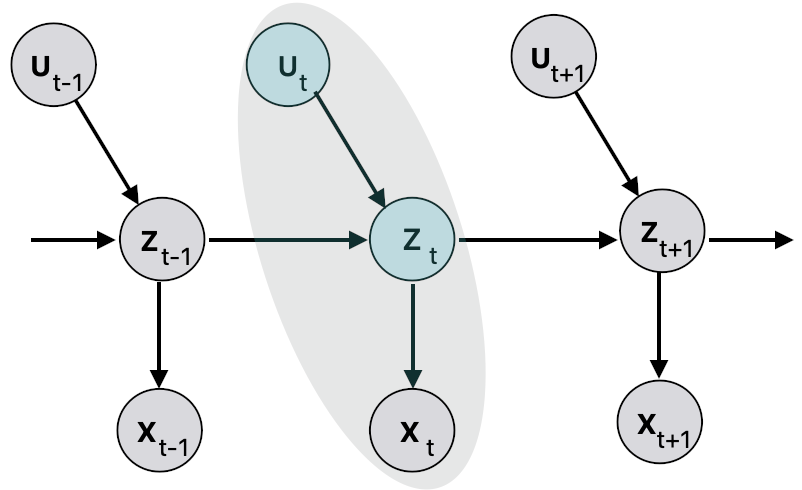
\includegraphics[width=200px]{./Images/dkf_model.png}
    \caption{DKF model as a Bayesian network. The inputs
    $\mathbf{u}_t$ are always observed.}
    \label{fig:dkf_model}
\end{figure}

\subsection{Generative model}\label{seq:generative_model}

The generative model is the joint distribution of observations and
latent states given the inputs,
$p(\mathbf{x}_{1:T}, \mathbf{z}_{1:T} \mid \mathbf{u}_{1:T})$. Ordering
the variables in time and applying the product rule,
\begin{align*}
    p(\mathbf{x}_{1:T}, \mathbf{z}_{1:T} \mid \mathbf{u}_{1:T})
    &= \prod_{t=1}^T p(\mathbf{x}_t, \mathbf{z}_t \mid \mathbf{x}_{1:t-1},
       \mathbf{z}_{1:t-1}, \mathbf{u}_{1:T}) \\
    &= \prod_{t=1}^T p(\mathbf{x}_t \mid \mathbf{x}_{1:t-1},
       \mathbf{z}_{1:t}, \mathbf{u}_{1:T})\,
       p(\mathbf{z}_t \mid \mathbf{x}_{1:t-1}, \mathbf{z}_{1:t-1},
       \mathbf{u}_{1:T}).
\end{align*}
The graph of Figure~\ref{fig:dkf_model} then simplifies each factor.
Using d-separation (Annex~\ref{seq:d_separation}):
\begin{itemize}
    \item $\mathbf{z}_{t} \indep (\mathbf{x}_{1:t-1},
    \mathbf{z}_{1:t-2}, \mathbf{u}_{1:t-1}, \mathbf{u}_{t+1:T}) \mid
    \mathbf{z}_{t-1}, \mathbf{u}_t$: every path from the past to
    $\mathbf{z}_t$ goes through $\mathbf{z}_{t-1}$, as a chain node or a
    fork node, and $\mathbf{z}_{t-1}$ is given. Future inputs only reach
    $\mathbf{z}_t$ through colliders on unobserved future states.
    \item $\mathbf{x}_{t} \indep (\mathbf{x}_{1:t-1}, \mathbf{z}_{1:t-1},
    \mathbf{u}_{1:T}) \mid \mathbf{z}_{t}$: $\mathbf{z}_t$ is the only
    parent of $\mathbf{x}_t$, and every path into $\mathbf{x}_t$ goes
    through it.
\end{itemize}
Hence\footnote{For $t=1$, $p(\mathbf{z}_t \mid \mathbf{z}_{t-1},
\mathbf{u}_{t})$ stands for $p(\mathbf{z}_1 \mid \mathbf{z}_0,
\mathbf{u}_{1})$, the prior on $\mathbf{z}_1$.}
\begin{equation}
    p(\mathbf{x}_{1:T}, \mathbf{z}_{1:T} \mid \mathbf{u}_{1:T}) =
    \prod_{t=1}^T p(\mathbf{x}_t \mid \mathbf{z}_{t})\,
    p(\mathbf{z}_t \mid \mathbf{z}_{t-1}, \mathbf{u}_{t}).
    \label{eq:generative_model}
\end{equation}

\section{The posterior and the inference model}\label{sec:posterior}

Learning a \emph{causal} generative model does not require \emph{causal}
inference. To infer $\mathbf{z}_t$ we may use all observations, past and
future, exactly as a Kalman smoother does.

\subsection{The four inference models of the paper}

Krishnan et al.\ \cite{krishnan2015deep} experiment with four
variational models:
\begin{itemize}
    \item \textbf{q-INDEP}: $q(\mathbf{z}_t \mid \mathbf{x}_t,
    \mathbf{u}_t)$, parameterised by a multi-layer perceptron (MLP);
    \item \textbf{q-LR}: $q(\mathbf{z}_t \mid \mathbf{x}_{t-1},
    \mathbf{x}_t, \mathbf{x}_{t+1}, \mathbf{u}_{t-1}, \mathbf{u}_t,
    \mathbf{u}_{t+1})$, parameterised by an MLP;
    \item \textbf{q-RNN}: $q(\mathbf{z}_t \mid \mathbf{x}_{1:t},
    \mathbf{u}_{1:t})$, parameterised by a recurrent neural network (RNN);
    \item \textbf{q-BRNN}: $q(\mathbf{z}_t \mid \mathbf{x}_{1:T},
    \mathbf{u}_{1:T})$, parameterised by a bidirectional RNN.
\end{itemize}
None of these conditions on the previous latent state: the latent
states are independent given the observations. Such \emph{mean-field}
approximations cannot represent the strong correlation between
successive states of the true posterior. The same paper, however, writes
the posterior in its structured form (its Equation~3), and the authors'
follow-up work \cite{krishnan2017structured} builds an inference network
of exactly that form, with a \enquote{combiner} that merges
$\mathbf{z}_{t-1}$ with an RNN summary of the observations. My
implementation follows the structured form, derived next.

\subsection{Structure of the true posterior}

By the product rule,
\[
    p_{\theta}(\mathbf{z}_{1:T} \mid \mathbf{x}_{1:T}, \mathbf{u}_{1:T})
    = \prod_{t=1}^T p_{\theta}(\mathbf{z}_t \mid \mathbf{z}_{1:t-1},
    \mathbf{x}_{1:T}, \mathbf{u}_{1:T}).
\]
Given $\mathbf{z}_{t-1}$, the past variables $\mathbf{z}_{1:t-2}$,
$\mathbf{x}_{1:t-1}$ and $\mathbf{u}_{1:t-1}$ are d-separated from
$\mathbf{z}_{t}$: in the graph, every path from them to $\mathbf{z}_t$
passes through $\mathbf{z}_{t-1}$ as a chain node or a fork node, and
observing $\mathbf{x}$ or $\mathbf{u}$ cannot open a path, because no
$\mathbf{x}$ or $\mathbf{u}$ node is a collider on such a path. The
future observations $\mathbf{x}_{t:T}$, on the other hand, remain
dependent on $\mathbf{z}_t$. Therefore
\begin{equation*}
    p_{\theta}(\mathbf{z}_{1:T} \mid \mathbf{x}_{1:T}, \mathbf{u}_{1:T})
    = \prod_{t=1}^T p_{\theta}\big(\mathbf{z}_t \mid
    \mathbf{z}_{t-1}, \mathbf{x}_{\textcolor{blue}{t}:T},
    \mathbf{u}_{\textcolor{blue}{t}:T}\big),
\end{equation*}
and it is natural to choose an inference model with the same structure:
\begin{equation}
    q_{\phi}(\mathbf{z}_{1:T} \mid \mathbf{x}_{1:T}, \mathbf{u}_{1:T}) =
    \prod_{t=1}^T q_{\phi}\big(\mathbf{z}_t \mid \mathbf{z}_{t-1},
    \mathbf{x}_{\textcolor{blue}{t}:T},
    \mathbf{u}_{\textcolor{blue}{t}:T}\big).
    \label{q_phi}
\end{equation}

\begin{inwords}
Once you know where the state was at time $t-1$, the past observations
have nothing more to tell you about the state at time $t$: their
information has been \enquote{absorbed} by $\mathbf{z}_{t-1}$. The
future observations, however, still matter, because they were generated
from states that $\mathbf{z}_t$ influences. So the posterior factor for
$\mathbf{z}_t$ needs exactly two ingredients: the previous state and a
summary of the observations from $t$ to $T$. The inference network is
built to receive exactly these two ingredients, and nothing else.
\end{inwords}

\begin{story}[{Notation for $t=1$}]
To keep formulas short, I write $p_{\theta}(\mathbf{z}_{t} \mid
\mathbf{z}_{t-1}, \star)$ and $q_{\phi}(\mathbf{z}_{t} \mid
\mathbf{z}_{t-1}, \star)$ also for $t = 1$, where $\mathbf{z}_0$ is the
fixed or learned initial value. Thus $p_{\theta}(\mathbf{z}_{1} \mid
\mathbf{z}_{0}, \star)$ is the prior on $\mathbf{z}_{1}$.
\end{story}

\section{Evidence Lower Bound}\label{sec:elbo}

The ELBO has the same definition as for the VAE, with the whole sequence
in place of a single data point:
\begin{align*}
    \mathcal{L}(\theta, \phi; \mathbf{x}_{1:T}, \mathbf{u}_{1:T}) =
    \E_{q_\phi(\mathbf{z}_{1:T} \mid \mathbf{x}_{1:T}, \mathbf{u}_{1:T})}
    \left[ \log \frac{p_\theta(\mathbf{x}_{1:T}, \mathbf{z}_{1:T} \mid
    \mathbf{u}_{1:T})}{q_\phi(\mathbf{z}_{1:T} \mid \mathbf{x}_{1:T},
    \mathbf{u}_{1:T})} \right]
    \;\leq\; \log p_\theta(\mathbf{x}_{1:T} \mid \mathbf{u}_{1:T}),
\end{align*}
and, as in \eqref{eq:elbo_gap}, the gap is
$\KL\big(q_\phi(\mathbf{z}_{1:T} \mid \mathbf{x}_{1:T}, \mathbf{u}_{1:T})
\,\|\, p_\theta(\mathbf{z}_{1:T} \mid \mathbf{x}_{1:T},
\mathbf{u}_{1:T})\big)$. Substituting the factorisations
\eqref{eq:generative_model} and \eqref{q_phi}, Appendix~\ref{sec:elbo_derivation}
shows that
\begin{equation}
\boxed{
\begin{aligned}
    \mathcal{L}(\theta, \phi) =\ &
    \sum_{t=1}^T \E_{q_{\phi}(\mathbf{z}_{t} \mid \mathbf{x}_{1:T},
    \mathbf{u}_{1:T})} \big[\log p_\theta(\mathbf{x}_t \mid
    \mathbf{z}_{t})\big] \\
    & - \sum_{t=1}^T \E_{q_\phi(\mathbf{z}_{t-1} \mid \mathbf{x}_{1:T},
    \mathbf{u}_{1:T})} \Big[ \KL\big( q_\phi(\mathbf{z}_t \mid
    \mathbf{z}_{t-1}, \mathbf{x}_{t:T}, \mathbf{u}_{t:T}) \,\big\|\,
    p_\theta(\mathbf{z}_t \mid \mathbf{z}_{t-1}, \mathbf{u}_{t}) \big)
    \Big]
\end{aligned}
}
\label{eq:dkf_elbo}
\end{equation}
where, for $t = 1$, the outer expectation is trivial because
$\mathbf{z}_0$ is fixed.
\begin{itemize}
    \item The \textbf{reconstruction term} measures how well each
    observation is explained by its latent state.
    \item The \textbf{regularisation term} measures, at each time step,
    how far the inference network's distribution for $\mathbf{z}_t$ is
    from what the dynamics predict from $\mathbf{z}_{t-1}$.
\end{itemize}

\begin{inwords}
The KL divergence between two distributions over whole trajectories
splits into one KL per time step: this is the \emph{chain rule} of the
KL divergence, and it holds because both the model and the inference
network are Markov chains. Each per-step KL compares two Gaussians for
$\mathbf{z}_t$ \emph{given} $\mathbf{z}_{t-1}$, so it has a closed form,
however complicated the neural networks are. The price is the outer
expectation over $\mathbf{z}_{t-1}$, which Section~\ref{sec:approximation_elbo}
shows how to handle.
\end{inwords}

\section{DKF Inference Model Design}

The datasets used in this project have no control input, so from now on
$\mathbf{u}$ is dropped:
\begin{equation*}
    q_{\phi}(\mathbf{z}_{1:T} \mid \mathbf{x}_{1:T}) =
    \prod_{t=1}^T q_{\phi}(\mathbf{z}_t \mid \mathbf{z}_{t-1},
    \mathbf{x}_{t:T}).
\end{equation*}
Each factor is a Gaussian with diagonal covariance,
\begin{equation*}
    q_{\phi}(\mathbf{z}_t \mid \mathbf{z}_{t-1}, \mathbf{x}_{t:T}) =
    \mathcal{N}\big(\mathbf{z}_t;\ \boldsymbol{\mu}_{\phi}(\mathbf{z}_{t-1},
    \mathbf{x}_{t:T}),\ \mathrm{diag}(\boldsymbol{\sigma}^2_{\phi}
    (\mathbf{z}_{t-1}, \mathbf{x}_{t:T}))\big),
\end{equation*}
whose parameters are computed by neural networks\footnote{The networks
output $\log \boldsymbol{\sigma}^2$ rather than $\boldsymbol{\sigma}^2$,
so that the variance, obtained with an exponential, is always
positive.}. The dependence on the whole suffix $\mathbf{x}_{t:T}$ is
handled by a \textbf{backward RNN} (an LSTM run from $T$ down to $1$,
Appendix~\ref{sec:backward_lstm}): its output at time $t$, written
$\mathbf{b}_t$, summarises $\mathbf{x}_{t:T}$
(Figure~\ref{fig:backward_rnn}). At each time step, a \textbf{combiner}
(Appendix~\ref{combiner_info}) merges $\mathbf{z}_{t-1}$ with
$\mathbf{b}_t$, and an MLP, the \textbf{encoder}, maps the result to
$\boldsymbol{\mu}_{\phi}$ and $\log \boldsymbol{\sigma}^2_{\phi}$.

\begin{figure}[ht!]
    \centering
    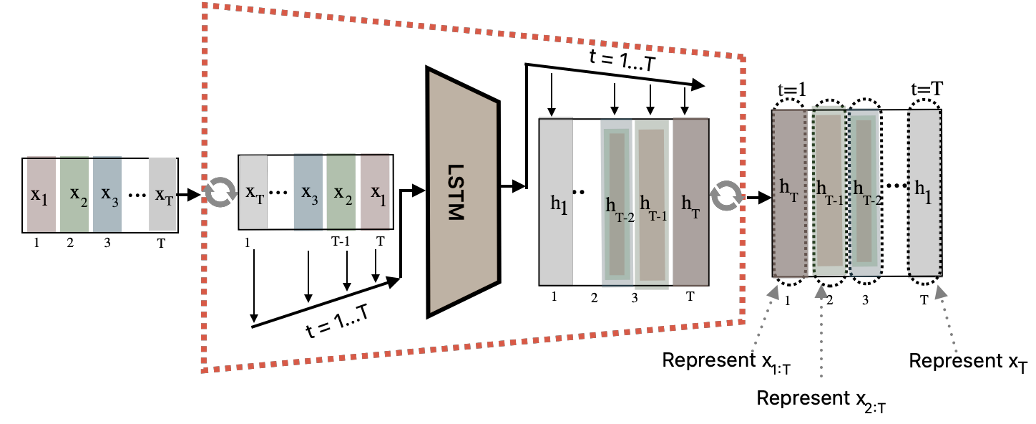
\includegraphics[width=400px]{./Images/backward_lstm.png}
    \caption{Backward RNN: the output at position $t$ summarises
    $\mathbf{x}_{t:T}$.}
    \label{fig:backward_rnn}
\end{figure}

\subsection{Reparameterisation trick}

As in the VAE, $\mathbf{z}_t$ is sampled as
\begin{equation*}
    \mathbf{z}_t = \boldsymbol{\mu}_{\phi}(\mathbf{z}_{t-1},
    \mathbf{x}_{t:T}) + \boldsymbol{\sigma}_{\phi}(\mathbf{z}_{t-1},
    \mathbf{x}_{t:T}) \odot \boldsymbol{\epsilon}_t,
    \qquad \boldsymbol{\epsilon}_t \sim \mathcal{N}(\mathbf{0},
    \mathbf{I}),
\end{equation*}
with $\boldsymbol{\sigma}_{\phi}$ the vector of standard deviations.
Note that $\mathbf{z}_{t-1}$ is itself a sample, so $\mathbf{z}_t$ is a
differentiable function of $\phi$ and of all the noises
$\boldsymbol{\epsilon}_1, \dots, \boldsymbol{\epsilon}_t$.

\subsection{Overall design}

The whole inference model is shown in Figure~\ref{fig:dkf_inference}.

\begin{figure}[ht!]
    \centering
    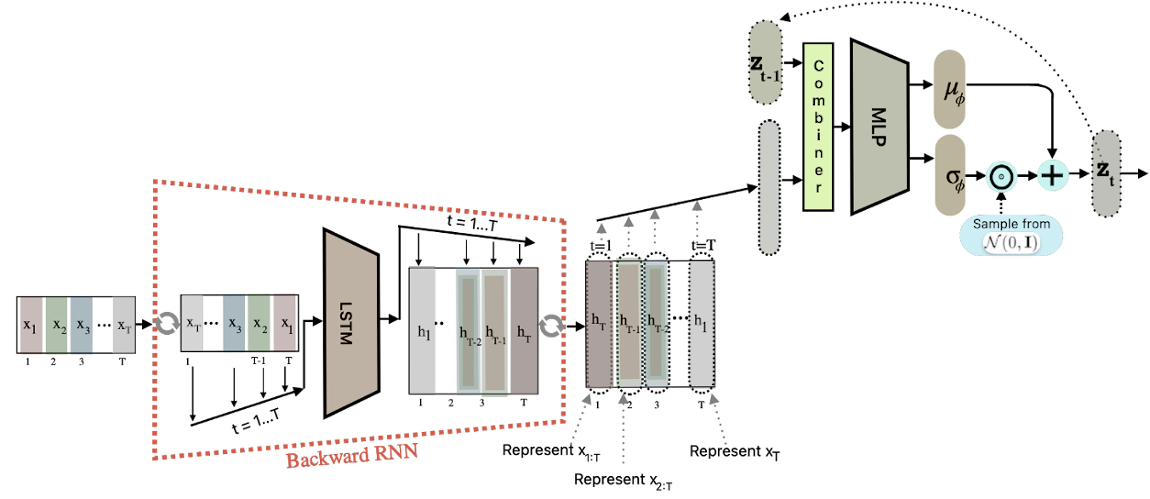
\includegraphics[width=450px]{./Images/dkf_detailed_inference.png}
    \caption{DKF inference model}
    \label{fig:dkf_inference}
\end{figure}

\section{DKF Generative Model Design}

Without control input, the generative model \eqref{eq:generative_model}
reads
\begin{equation}
    p_{\theta}(\mathbf{x}_{1:T}, \mathbf{z}_{1:T}) =
    \prod_{t=1}^T p_{\theta_{\mathbf{x}}}(\mathbf{x}_t \mid \mathbf{z}_{t})
    \,p_{\theta_{\mathbf{z}}}(\mathbf{z}_t \mid \mathbf{z}_{t-1}),
    \label{eq:recall_generative_model}
\end{equation}
with diagonal Gaussians for both factors.

\paragraph{Transition model.}
\begin{equation*}
    p_{\theta_{\mathbf{z}}}(\mathbf{z}_t \mid \mathbf{z}_{t-1}) =
    \mathcal{N}\big(\mathbf{z}_t;\ \boldsymbol{\mu}_{\theta_{\mathbf{z}}}
    (\mathbf{z}_{t-1}),\ \mathrm{diag}(\boldsymbol{\sigma}^2_{
    \theta_{\mathbf{z}}}(\mathbf{z}_{t-1}))\big).
\end{equation*}

\paragraph{Emission (reconstruction) model.}
\begin{equation*}
    p_{\theta_{\mathbf{x}}}(\mathbf{x}_t \mid \mathbf{z}_{t}) =
    \mathcal{N}\big(\mathbf{x}_t;\ \boldsymbol{\mu}_{\theta_{\mathbf{x}}}
    (\mathbf{z}_{t}),\ \mathrm{diag}(\boldsymbol{\sigma}^2_{
    \theta_{\mathbf{x}}}(\mathbf{z}_{t}))\big).
\end{equation*}

Both pairs of parameters are computed by MLPs
(Figure~\ref{fig:dkf_generative}), which again output
$\log\boldsymbol{\sigma}^2$.

\begin{figure}[ht!]
    \centering
    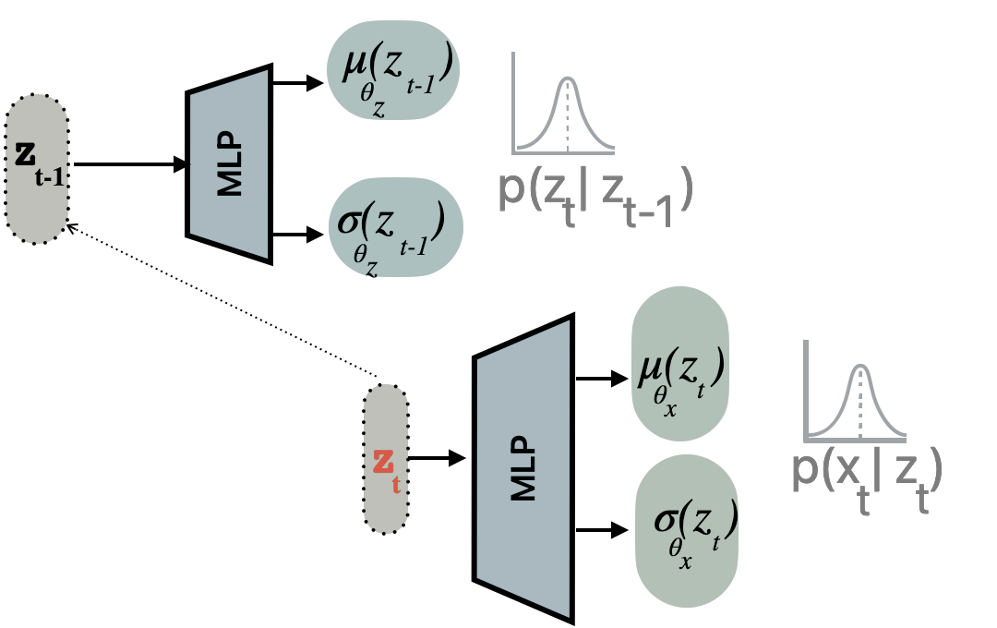
\includegraphics[width=250px]{./Images/dkf_generative.png}
    \caption{DKF generative model}
    \label{fig:dkf_generative}
\end{figure}

\begin{story}[Reconstruction]
Given a latent state $\mathbf{z}_t$, the most likely observation is the
mean $\hat{\mathbf{x}}_{t} = \boldsymbol{\mu}_{\theta_{\mathbf{x}}}
(\mathbf{z}_{t})$. This is what I call the \enquote{reconstruction} of
$\mathbf{x}_t$ in the experiments.
\end{story}

%~~~~~~~~~~~~~~~~~~~~~~~~~~~~~~~~~~~~~~~~~~~~~~~~~~~~~~~~~~~~~~~~~~~~~~~~
\section{Estimating the ELBO}\label{sec:approximation_elbo}

\subsection{The difficulty}

Both terms of \eqref{eq:dkf_elbo} are expectations under
\emph{marginals} of the inference model,
$q_\phi(\mathbf{z}_{t} \mid \mathbf{x}_{1:T})$ and
$q_\phi(\mathbf{z}_{t-1} \mid \mathbf{x}_{1:T})$. These marginals are
intractable: for instance
\[
    q_\phi(\mathbf{z}_{t} \mid \mathbf{x}_{1:T}) = \int
    q_\phi(\mathbf{z}_{t} \mid \mathbf{z}_{t-1}, \mathbf{x}_{t:T})\,
    q_\phi(\mathbf{z}_{t-1} \mid \mathbf{x}_{1:T})\,d\mathbf{z}_{t-1}
\]
is an integral over all the earlier latent states. With non-linear
networks it is not Gaussian, and in general it has no closed form at all.

\subsection{Ancestral sampling}

We never need the \emph{density} of these marginals, only
\emph{samples} from them. Draw one trajectory by ancestral sampling:
\begin{equation*}
    \dot{\mathbf{z}}_1 \sim q_\phi(\mathbf{z}_1 \mid \mathbf{z}_0,
    \mathbf{x}_{1:T}),\quad
    \dot{\mathbf{z}}_2 \sim q_\phi(\mathbf{z}_2 \mid \dot{\mathbf{z}}_1,
    \mathbf{x}_{2:T}),\quad \dots,\quad
    \dot{\mathbf{z}}_T \sim q_\phi(\mathbf{z}_T \mid
    \dot{\mathbf{z}}_{T-1}, \mathbf{x}_{T}).
\end{equation*}
By \eqref{q_phi}, the trajectory $\dot{\mathbf{z}}_{1:T}$ is an exact
sample from the joint $q_\phi(\mathbf{z}_{1:T} \mid \mathbf{x}_{1:T})$.
Consequently, each $\dot{\mathbf{z}}_t$ is an exact sample from the
marginal $q_\phi(\mathbf{z}_{t} \mid \mathbf{x}_{1:T})$. One trajectory
provides samples of every marginal at once.

\subsection{The estimator}

Evaluate both terms of \eqref{eq:dkf_elbo} along the sampled trajectory:
\begin{equation}
    \hat{\mathcal{L}} = \sum_{t=1}^T \log p_\theta(\mathbf{x}_t \mid
    \dot{\mathbf{z}}_t) - \sum_{t=1}^T \KL\big(q_\phi(\mathbf{z}_t \mid
    \dot{\mathbf{z}}_{t-1}, \mathbf{x}_{t:T}) \,\big\|\,
    p_\theta(\mathbf{z}_t \mid \dot{\mathbf{z}}_{t-1})\big),
    \label{eq:elbo_estimator}
\end{equation}
where each KL is computed in closed form
(Appendix~\ref{sec:elbo_regularization}) at the sampled
$\dot{\mathbf{z}}_{t-1}$.

\begin{proposition}\label{prop:unbiased}
$\E\big[\hat{\mathcal{L}}\big] = \mathcal{L}(\theta, \phi;
\mathbf{x}_{1:T})$: the single-trajectory estimator is unbiased.
\end{proposition}
\begin{proof}
By linearity of expectation it is enough to treat each term. Since
$\dot{\mathbf{z}}_t \sim q_\phi(\mathbf{z}_{t} \mid \mathbf{x}_{1:T})$,
$\E[\log p_\theta(\mathbf{x}_t \mid \dot{\mathbf{z}}_t)] =
\E_{q_\phi(\mathbf{z}_{t} \mid \mathbf{x}_{1:T})}[\log
p_\theta(\mathbf{x}_t \mid \mathbf{z}_t)]$. Likewise, since
$\dot{\mathbf{z}}_{t-1} \sim q_\phi(\mathbf{z}_{t-1} \mid
\mathbf{x}_{1:T})$, the expectation of the $t$-th KL term is the
expectation of the KL under $q_\phi(\mathbf{z}_{t-1} \mid
\mathbf{x}_{1:T})$. These are exactly the terms of \eqref{eq:dkf_elbo}.
\end{proof}

\begin{inwords}
Each term of the ELBO is an average of something over the latent states.
Averages can be estimated by plugging in samples, and nothing non-linear
is applied to those averages afterwards. So one sampled trajectory gives
an estimate that is right on average: some trajectories overshoot, some
undershoot, and the errors cancel in expectation. That is what makes
training with one trajectory per sequence legitimate. Averaging over the
sequences of a minibatch then reduces the noise.
\end{inwords}

A numerical demonstration of Proposition~\ref{prop:unbiased}, on a
model where the ELBO can be computed exactly, is in the notebook
\href{https://github.com/CL-BZH/Deep-Kalman-Filters/blob/main/Notebooks/elbo_expectations.ipynb}{\texttt{elbo\_expectations.ipynb}}.

\subsection{Why compute the KL terms in closed form?}

One could also estimate the regularisation term by sampling, using
$\log q_\phi(\dot{\mathbf{z}}_t \mid \dot{\mathbf{z}}_{t-1},
\mathbf{x}_{t:T}) - \log p_\theta(\dot{\mathbf{z}}_t \mid
\dot{\mathbf{z}}_{t-1})$ in place of each KL. That is also unbiased.
Computing the KL in closed form instead integrates $\mathbf{z}_t$ out
exactly given $\dot{\mathbf{z}}_{t-1}$. This is
\emph{Rao--Blackwellisation}, and by the law of total variance it lowers
the variance of each KL term. Krishnan et al.\ report that sampling the
KL term gives high-variance gradients, which motivates this choice.

Two remarks are worth making. First, the factorisation
\eqref{eq:dkf_elbo} is what makes a closed form possible at all: the KL
between two distributions over whole trajectories has no closed form
when the transition is a neural network, while each per-step KL is
between two diagonal Gaussians. Second, lower variance for each term
does not guarantee lower variance for the whole estimate, because the
sampled terms are correlated. In the experiments of the notebook cited
above, the closed-form KL gave less noisy gradients for every encoder
tried, but the sampled version gave a less noisy \emph{value} of the
ELBO when the encoder was close to the true posterior.

\subsection{Differentiability}

With the reparameterisation trick, $\hat{\mathcal{L}}$ is a
differentiable function of $\theta$ and $\phi$ for fixed noises
$\boldsymbol{\epsilon}_{1:T}$, and its gradient is an unbiased estimate
of $\nabla\mathcal{L}$. This is all stochastic gradient descent needs.

%~~~~~~~~~~~~~~~~~~~~~~~~~~~~~~~~~~~~~~~~~~~~~~~~~~~~~~~~~~~~~~~~~~~~~~~~
\section{Training the DKF}\label{sec:training}

The DKF is trained by minimising $-\hat{\mathcal{L}}$, averaged over a
minibatch of sequences, with respect to $\theta_{\mathbf{x}}$,
$\theta_{\mathbf{z}}$ and $\phi$, using the Adam optimiser. The complete
model is shown in Figure~\ref{fig:dkf}.

\begin{figure}[ht!]
    \centering
    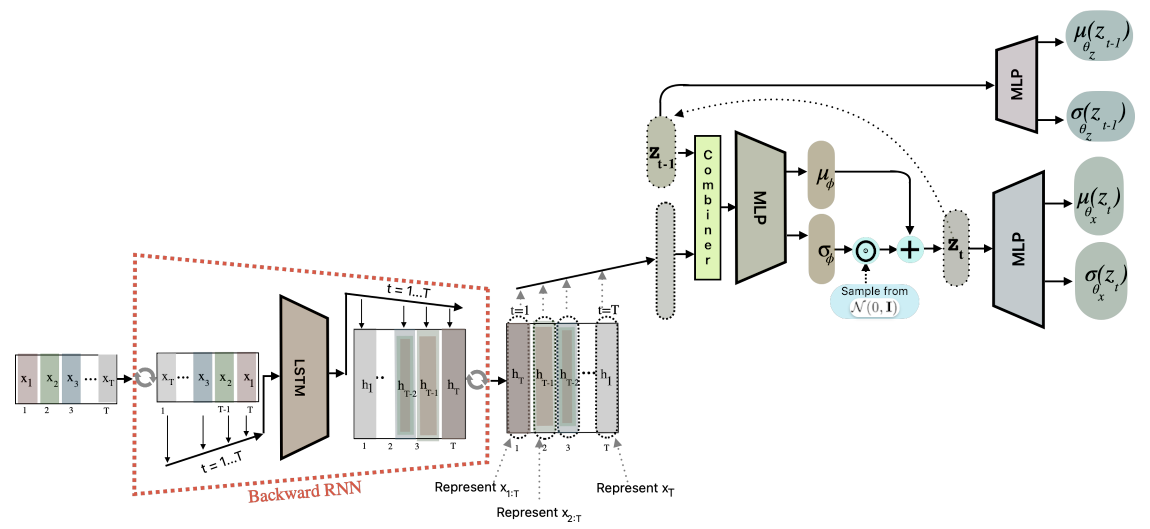
\includegraphics[width=460px]{./Images/dkf.png}
    \caption{DKF model: inference network (left and centre) and
    generative networks (right).}
    \label{fig:dkf}
\end{figure}

\subsection*{One training step}

\begin{enumerate}
    \item \textbf{Summarise the future.} Run the backward RNN over
    $\mathbf{x}_{1:T}$ to obtain $\mathbf{b}_1, \dots, \mathbf{b}_T$,
    where $\mathbf{b}_t$ summarises $\mathbf{x}_{t:T}$.

    \item \textbf{Sample a latent trajectory (ancestral sampling).} For
    $t = 1, \dots, T$: combine $\dot{\mathbf{z}}_{t-1}$ with
    $\mathbf{b}_t$, compute $\boldsymbol{\mu}_{\phi}$ and
    $\log\boldsymbol{\sigma}^2_{\phi}$ with the encoder, and draw
    $\dot{\mathbf{z}}_t$ with the reparameterisation trick.

    \item \textbf{Evaluate the transition.} For each $t$, compute
    $\boldsymbol{\mu}_{\theta_{\mathbf{z}}}(\dot{\mathbf{z}}_{t-1})$ and
    $\log\boldsymbol{\sigma}^2_{\theta_{\mathbf{z}}}
    (\dot{\mathbf{z}}_{t-1})$ at the \emph{sampled} previous state.

    \item \textbf{Decode.} For each $t$, compute
    $\boldsymbol{\mu}_{\theta_{\mathbf{x}}}(\dot{\mathbf{z}}_{t})$ and
    $\log\boldsymbol{\sigma}^2_{\theta_{\mathbf{x}}}(\dot{\mathbf{z}}_{t})$.

    \item \textbf{Compute the loss} $-\hat{\mathcal{L}}$
    (Section~\ref{sec:loss}).

    \item \textbf{Update.} Backpropagate through the whole computation,
    including the sampling steps thanks to the reparameterisation trick,
    and take one optimiser step.
\end{enumerate}

\subsection{The loss function}\label{sec:loss}

Using \eqref{eq:sum_log_p_theta_x_given_z} (Appendix~\ref{sec:elbo_recon})
and \eqref{eq:regularization_term}
(Appendix~\ref{sec:elbo_regularization}), and writing $d_x$ and $d_z$ for
the dimensions of $\mathbf{x}_t$ and $\mathbf{z}_t$,
\begin{align*}
    -\sum_{t=1}^T \log p_{\theta_{\mathbf{x}}}(\mathbf{x}_t \mid
    \dot{\mathbf{z}}_{t}) &= \frac{T d_x}{2} \log(2\pi) +
    \frac{1}{2} \sum_{t=1}^T \sum_{i=1}^{d_x} \left[ \log
    \sigma^2_{\theta_{\mathbf{x}}, i}(\dot{\mathbf{z}}_{t}) +
    \frac{\big(x_{t,i} - \mu_{\theta_{\mathbf{x}}, i}(\dot{\mathbf{z}}_{t})
    \big)^2}{\sigma^2_{\theta_{\mathbf{x}}, i}(\dot{\mathbf{z}}_{t})}
    \right], \\
    \sum_{t=1}^T \KL_t &= -\frac{T d_z}{2} + \frac{1}{2} \sum_{t=1}^T
    \sum_{i=1}^{d_z} \left[ \frac{\sigma^2_{\phi, i} + (\mu_{\theta_{
    \mathbf{z}}, i} - \mu_{\phi, i})^2}{\sigma^2_{\theta_{\mathbf{z}},
    i}} + \log \sigma^2_{\theta_{\mathbf{z}}, i} - \log \sigma^2_{\phi,
    i} \right],
\end{align*}
where, in the second line, the parameters of $q_\phi$ are evaluated at
$(\dot{\mathbf{z}}_{t-1}, \mathbf{x}_{t:T})$ and those of
$p_{\theta_{\mathbf{z}}}$ at $\dot{\mathbf{z}}_{t-1}$. The constants
$\frac{T d_x}{2}\log(2\pi)$ and $-\frac{T d_z}{2}$ do not depend on the
parameters and can be dropped. This leaves the two losses

\begin{center}
\boxed{
    \mathcal{L}_{\text{rec}} = \frac{1}{2} \sum_{t=1}^T
    \sum_{i=1}^{d_x} \left[ \log \sigma^2_{\theta_{\mathbf{x}}, i} +
    \frac{(x_{t,i} - \mu_{\theta_{\mathbf{x}}, i})^2}
    {\sigma^2_{\theta_{\mathbf{x}}, i}} \right]
}
\qquad
\boxed{
    \mathcal{L}_{\text{reg}} = \frac{1}{2} \sum_{t=1}^T
    \sum_{i=1}^{d_z} \left[ \frac{\sigma^2_{\phi, i} +
    (\mu_{\theta_{\mathbf{z}}, i} - \mu_{\phi, i})^2}
    {\sigma^2_{\theta_{\mathbf{z}}, i}} + \log
    \sigma^2_{\theta_{\mathbf{z}}, i} - \log \sigma^2_{\phi, i}
    \right]
}
\end{center}
and $-\hat{\mathcal{L}} = \mathcal{L}_{\text{rec}} +
\mathcal{L}_{\text{reg}} + \text{const}$.

\begin{story}[What the code computes]
The function \code{loss\_function} in \code{Utils/loss\_fcts.py}
computes $\frac{2}{T}\big(\mathcal{L}_{\text{rec}} + \beta\,
\mathcal{L}_{\text{reg}}\big)$, averaged over the minibatch: the factor
$\frac12$ is omitted and the result is divided by the sequence length.
Neither changes the minimiser. With $\beta = 1$ this is exactly the
negative ELBO estimate \eqref{eq:elbo_estimator}, up to a constant and a
positive factor. With $\beta \neq 1$ the objective is a weighted
($\beta$-VAE-style) variant. The option \code{loss\_type='mse'} drops the
decoder variance, so its reconstruction term is no longer a
log-likelihood and the objective is no longer an ELBO.
\end{story}

%~~~~~~~~~~~~~~~~~~~~~~~~~~~~~~~~~~~~~~~~~~~~~~~~~~~~~~~~~~~~~~~~~~~~~~~~
\section{Implementation}

The main classes of the implementation\footnote{The code is available
\href{https://github.com/CL-BZH/Deep-Kalman-Filters/tree/main}{on
GitHub}.} are shown in Figure~\ref{fig:dkf_implementation_objects}.

\begin{figure}[ht!]
    \centering
    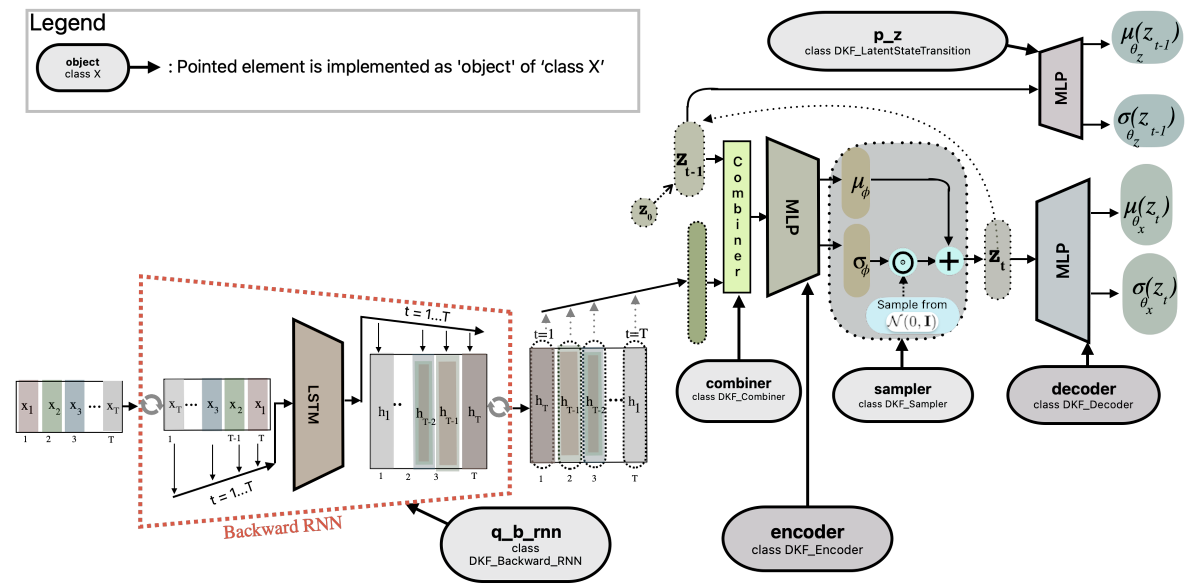
\includegraphics[width=460px]{./Images/dkf_implementation_objects.png}
    \caption{DKF implementation classes}
    \label{fig:dkf_implementation_objects}
\end{figure}

\subsection{The forward pass}

The \code{forward} method of the \code{DKF} class implements steps 1 to
4 of the training procedure for a minibatch of sequences
$\mathbf{x}$ of shape \code{(seq\_len, batch\_size, x\_dim)}.
\begin{enumerate}
    \item \textbf{Initial state.} $\mathbf{z}_0$ is the learnable
    parameter \code{Z\_0} if \code{learnable\_init\_z=True}, and a tensor
    of zeros otherwise. It is expanded to the batch size.
    \item \textbf{Backward RNN.} $\mathbf{x}$ is passed through the
    backward RNN \code{q\_b\_rnn}, which returns
    $\mathbf{b}_1, \dots, \mathbf{b}_T$.
    \item \textbf{Ancestral sampling.} For each $t$, the \code{combiner}
    merges the previous sample with $\mathbf{b}_t$, the \code{encoder}
    returns $\boldsymbol{\mu}_{\phi}$ and $\log\boldsymbol{\sigma}^2_{\phi}$,
    and the \code{sampler} draws $\dot{\mathbf{z}}_t$ with the
    reparameterisation trick. Means, log-variances and samples are
    stored.
    \item \textbf{Transition.} The transition network \code{p\_z} is
    applied to the shifted sequence
    $(\mathbf{z}_0, \dot{\mathbf{z}}_1, \dots, \dot{\mathbf{z}}_{T-1})$,
    giving the parameters of $p(\mathbf{z}_t \mid
    \dot{\mathbf{z}}_{t-1})$ for every $t$.
    \item \textbf{Decoding.} The \code{decoder} is applied to
    $\dot{\mathbf{z}}_{1:T}$ and returns
    $\hat{\mathbf{x}} = \boldsymbol{\mu}_{\theta_{\mathbf{x}}}$ and
    $\log\boldsymbol{\sigma}^2_{\theta_{\mathbf{x}}}$.
\end{enumerate}
It returns everything the loss function needs.

\subsection{The \texttt{predict} function}

\code{predict} takes an observed sequence $\mathbf{x}_{1:T}$ and returns
its reconstruction followed by \code{num\_steps} forecasts.
\begin{enumerate}
    \item It samples a latent trajectory $\dot{\mathbf{z}}_{1:T}$ exactly
    as in the forward pass, and decodes it to obtain the
    reconstruction.
    \item Starting from $\dot{\mathbf{z}}_T$, it repeatedly applies the
    transition model: it computes the parameters of
    $p(\mathbf{z}_{s} \mid \mathbf{z}_{s-1})$, samples
    $\mathbf{z}_{s}$, and decodes it into the forecast
    $\boldsymbol{\mu}_{\theta_{\mathbf{x}}}(\mathbf{z}_s)$.
\end{enumerate}

\begin{inwords}[Why this is the right way to forecast]
At the last time step, the inference network conditions only on
$\mathbf{z}_{T-1}$ and $\mathbf{x}_{T}$, so
$q_\phi(\mathbf{z}_T \mid \mathbf{x}_{1:T})$ approximates the
\emph{filtering} distribution $p(\mathbf{z}_T \mid \mathbf{x}_{1:T})$:
everything that has been observed, nothing more. Propagating samples of
it through the learned dynamics is the non-linear analogue of the Kalman
prediction step. Two limitations follow. A forecast is a single sampled
path, not the mean of the predictive distribution, so its error includes
the sampling noise. And the model can only forecast well if the
transition network has learned the dynamics. A very flexible inference
network can explain the training data while the transition network
stays poor (Appendix~\ref{sec:results}).
\end{inwords}

%======================================================================
\section{The Autoregressive DKF (AR DKF)}\label{sec:ar_dkf}

\subsection{Motivation}

On the sine-wave data, the vanilla DKF reconstructs the observed part of
a sequence well but fails to forecast it (Appendix~\ref{sec:results}).
Its forecasts depend only on the transition model
$p(\mathbf{z}_t \mid \mathbf{z}_{t-1})$, and nothing forces that model to
carry the information needed for long-range prediction. To give the
dynamics direct access to the history, I designed the
\enquote{Autoregressive} DKF (AR DKF), whose transition also depends on
the past observations:
\begin{equation*}
    p_{\theta_{\mathbf{z}}}(\mathbf{z}_t \mid \mathbf{z}_{t-1},
    \mathbf{x}_{0:t-1}),
\end{equation*}
where $\mathbf{x}_0$ is a fixed (zero) or learned initial value, so that
the transition into $\mathbf{z}_1$ is defined. In other words, the
independence $\mathbf{z}_t \indep \mathbf{x}_{1:t-1} \mid
\mathbf{z}_{t-1}$ of the vanilla DKF is given up on purpose by adding
edges from the past observations to $\mathbf{z}_t$
(Figure~\ref{fig:ar_dkf_transition_versus_dkf_transition}).

\begin{figure}[ht!]
    \centering
    \begin{minipage}{0.30\textwidth}
        \centering
        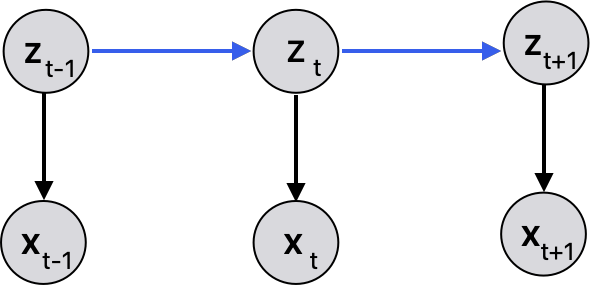
\includegraphics[width=1\textwidth]{./Images/dkf_transition_model.png}
        \subcaption{DKF model}
        \label{fig:dkf_transition_model}
    \end{minipage}
    \hspace{2cm}
    \begin{minipage}{0.30\textwidth}
        \centering
        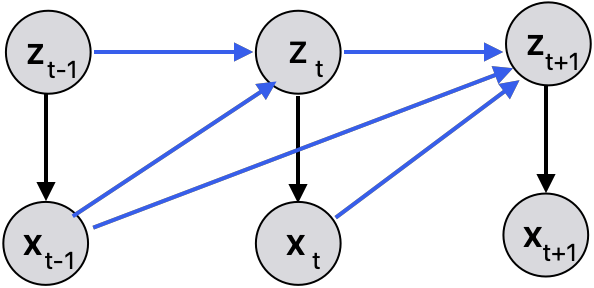
\includegraphics[width=1\textwidth]{./Images/ar_dkf_transition_model.png}
        \subcaption{AR DKF model}
        \label{fig:ar_dkf_transition_model}
    \end{minipage}
    \caption{DKF model versus AR DKF model (blue: the added edges).}
    \label{fig:ar_dkf_transition_versus_dkf_transition}
\end{figure}

\subsection{Generative model}

The joint distribution becomes
\begin{equation}
    p_{\theta}(\mathbf{x}_{1:T}, \mathbf{z}_{1:T}) =
    \prod_{t=1}^T p_{\theta_{\mathbf{x}}}(\mathbf{x}_t \mid \mathbf{z}_{t})
    \,p_{\theta_{\mathbf{z}}}(\mathbf{z}_t \mid \mathbf{z}_{t-1},
    \mathbf{x}_{0:t-1}).
    \label{eq:ar_generative}
\end{equation}
It is still a valid, causal generative model: each variable depends only
on variables generated before it. The history $\mathbf{x}_{0:t-1}$ is
summarised by a \textbf{forward RNN} (\code{pz\_f\_rnn}) run on the
shifted sequence $(\mathbf{x}_0, \mathbf{x}_1, \dots, \mathbf{x}_{T-1})$:
its output $\mathbf{h}_{t-1}$ summarises $\mathbf{x}_{0:t-1}$, and an MLP
maps $(\mathbf{z}_{t-1}, \mathbf{h}_{t-1})$ to the mean and log-variance
of the transition. The ELBO keeps the form \eqref{eq:dkf_elbo}, with
$p_{\theta_{\mathbf{z}}}(\mathbf{z}_t \mid \mathbf{z}_{t-1},
\mathbf{x}_{0:t-1})$ in the KL terms, and it is estimated in the same
way.

\subsection{What the new edges change for inference}\label{sec:ar_posterior}

Changing the generative model changes its posterior, and therefore the
inference network it needs. Redo the d-separation argument of
Section~\ref{sec:posterior} on the AR DKF graph.

\begin{proposition}\label{prop:ar_posterior}
In the AR DKF,
\begin{equation*}
    p_\theta(\mathbf{z}_{1:T} \mid \mathbf{x}_{1:T}) =
    \prod_{t=1}^T p_\theta(\mathbf{z}_t \mid \mathbf{z}_{t-1},
    \mathbf{x}_{\textcolor{red}{1}:T}),
\end{equation*}
and in general $p_\theta(\mathbf{z}_t \mid \mathbf{z}_{t-1},
\mathbf{x}_{1:T})$ depends on the past observations
$\mathbf{x}_{1:t-1}$ as well as on $\mathbf{x}_{t:T}$.
\end{proposition}
\begin{proof}
\emph{Earlier states drop out.} Take a path from $\mathbf{z}_s$, $s
\leq t-2$, to $\mathbf{z}_t$. Paths through the latent chain pass
through $\mathbf{z}_{t-1}$ as a chain or fork node and are blocked
because $\mathbf{z}_{t-1}$ is given. Any other path must pass through an
observation $\mathbf{x}_r$. Each observation has a single parent,
$\mathbf{z}_r$, so it can never be a collider on a path: the path passes
through $\mathbf{x}_r$ as a chain node ($\mathbf{z}_r \to \mathbf{x}_r
\to \mathbf{z}_{r'}$) or as a fork node ($\mathbf{z}_{r'} \leftarrow
\mathbf{x}_r \to \mathbf{z}_{r''}$). Since all observations are given,
such a path is blocked too.
\emph{Past observations do not drop out.} For $t \geq 2$,
$\mathbf{x}_{t-1}$ is a \emph{parent} of $\mathbf{z}_t$: the edge
$\mathbf{x}_{t-1} \to \mathbf{z}_t$ is a path of length one, with no
intermediate node that could block it. Hence no conditioning set can
make $\mathbf{z}_t$ independent of $\mathbf{x}_{t-1}$.
\end{proof}

\begin{inwords}
In the vanilla DKF, the past observations only influence $\mathbf{z}_t$
\emph{through} $\mathbf{z}_{t-1}$, so knowing $\mathbf{z}_{t-1}$ makes
them redundant. In the AR DKF they influence $\mathbf{z}_t$
\emph{directly}, through the new edges, so they can never become
redundant. The inference network for $\mathbf{z}_t$ must therefore see
the past observations as well as the future ones.
\end{inwords}

The AR DKF as implemented keeps the inference network of the vanilla
DKF, $q_\phi(\mathbf{z}_t \mid \mathbf{z}_{t-1}, \mathbf{x}_{t:T})$,
which ignores $\mathbf{x}_{1:t-1}$. By Proposition~\ref{prop:ar_posterior}
it cannot represent the true posterior, even with unlimited capacity, so
the gap $\KL(q_\phi \,\|\, p_\theta(\cdot \mid \mathbf{x}))$ in the ELBO
can never close. The variants of the next section repair this.

\subsection{Prediction}

Forecasting works as for the DKF, except that each transition step also
needs the summary $\mathbf{h}$ of the observations so far. After a
forecast $\hat{\mathbf{x}}_s$ is produced, it is appended to the
sequence and the forward RNN is run again, so that the next transition
step is conditioned on the model's own past forecasts. This makes the
AR DKF a genuinely autoregressive forecaster.

\begin{story}[A detail of the implementation]
In \code{predict}, the sequence fed to the forward RNN is a sliding
window: each new forecast is appended and the oldest observation is
removed, and the RNN is re-run from the start of the window. During
training, the RNN always starts from $\mathbf{x}_0$. The summaries seen
at prediction time are therefore computed slightly differently from
those seen during training.
\end{story}

The AR DKF design is shown in
Figure~\ref{fig:ar_dkf_implementation_objects}.

\begin{figure}[ht!]
    \centering
    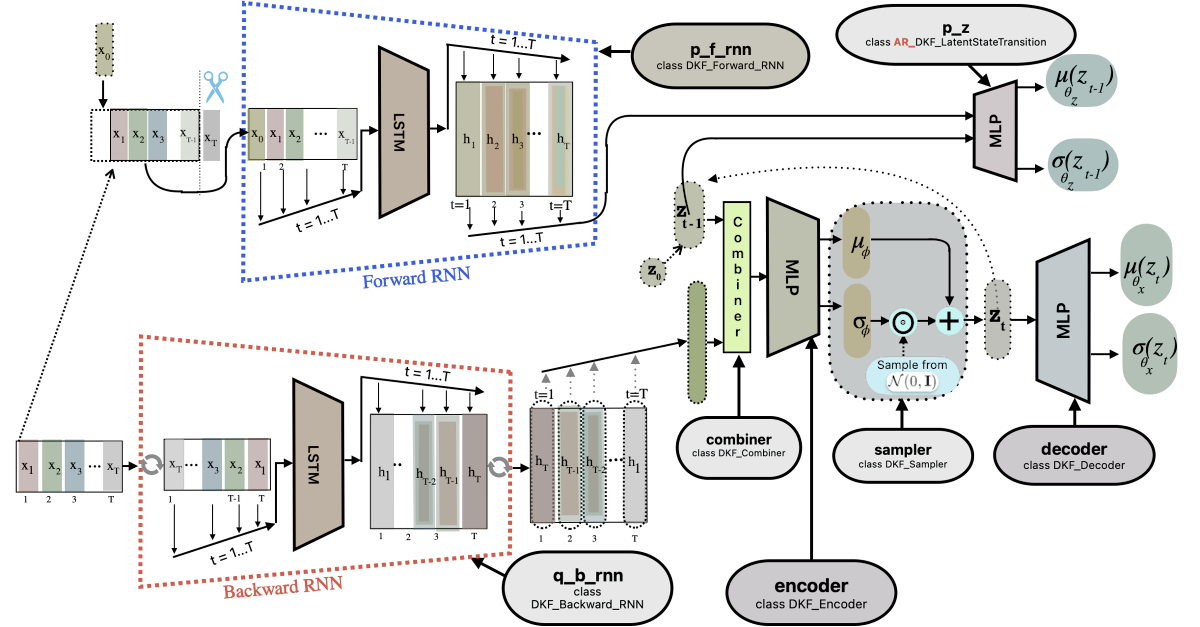
\includegraphics[width=480px]{./Images/ar_dkf_implementation_objects.png}
    \caption{AR DKF model}
    \label{fig:ar_dkf_implementation_objects}
\end{figure}

%- - - - - - - - - - - - - - - - - - - - - - - - - - - - - - - - - - - -
\section{The FAR DKF and BAR DKF models}\label{sec:far_bar}

The FAR DKF (\enquote{Forward Autoregressive}) and the BAR DKF
(\enquote{Bidirectional Autoregressive}) keep the generative model of the
AR DKF, including its transition $p_{\theta_{\mathbf{z}}}(\mathbf{z}_t
\mid \mathbf{z}_{t-1}, \mathbf{x}_{0:t-1})$, unchanged. They differ from it
only in the \textbf{inference network}, which in both variants receives
information about the past observations. By
Proposition~\ref{prop:ar_posterior}, this is exactly what the AR DKF
posterior requires.

\subsection{Forward Autoregressive DKF (FAR DKF)}

The FAR DKF adds a second forward RNN, \code{q\_f\_rnn}, to the inference
network (Figure~\ref{fig:far_dkf_implementation_objects}). Its output at
time $t$, $\overrightarrow{\mathbf{h}}_t$, summarises $\mathbf{x}_{1:t}$. The combiner
merges $\dot{\mathbf{z}}_{t-1}$ with both $\mathbf{b}_t$ (the future)
and $\overrightarrow{\mathbf{h}}_t$ (the past), so the inference model becomes
\begin{equation*}
    q_\phi(\mathbf{z}_t \mid \mathbf{z}_{t-1}, \mathbf{x}_{1:T}),
\end{equation*}
which has the structure of the true posterior of
Proposition~\ref{prop:ar_posterior}. The FAR DKF is therefore the
principled inference model for the AR DKF generative model. The linear
combiner offers separate weights for the two RNN summaries
(Appendix~\ref{combiner_info}).

\begin{figure}[ht!]
    \centering
    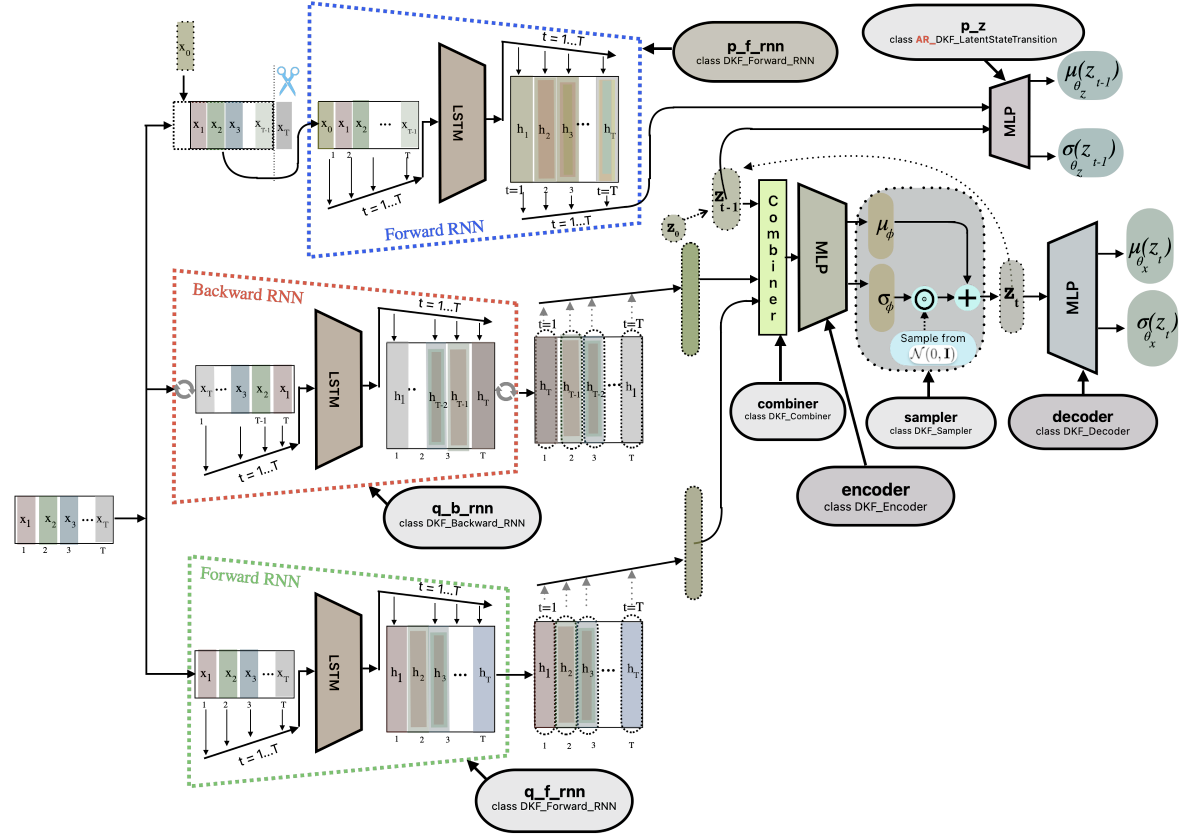
\includegraphics[width=480px]{./Images/far_dkf_implementation_objects.png}
    \caption{FAR DKF: the forward RNN \code{q\_f\_rnn} feeds the
    combiner of the inference network.}
    \label{fig:far_dkf_implementation_objects}
\end{figure}

\subsection{Bidirectional Autoregressive DKF (BAR DKF)}

The BAR DKF replaces the backward RNN of the inference network by a
single bidirectional RNN, whose output at time $t$ combines a summary of
$\mathbf{x}_{1:t}$ and a summary of $\mathbf{x}_{t:T}$. Its inference
model therefore also has the form $q_\phi(\mathbf{z}_t \mid
\mathbf{z}_{t-1}, \mathbf{x}_{1:T})$, with fewer parameters than the FAR
DKF because the two directions are merged before the combiner.

\subsection{Summary}

All three autoregressive variants share the generative model
\eqref{eq:ar_generative}. They differ in their inference networks:
\begin{center}
\begin{tabular}{|l|l|l|}
\hline
\textbf{Model} & \textbf{Inference network} & \textbf{Matches the
posterior structure?} \\ \hline
AR DKF & $q_\phi(\mathbf{z}_t \mid \mathbf{z}_{t-1}, \mathbf{x}_{t:T})$
& No: ignores $\mathbf{x}_{1:t-1}$ \\ \hline
FAR DKF & $q_\phi(\mathbf{z}_t \mid \mathbf{z}_{t-1}, \mathbf{x}_{1:T})$,
two RNNs & Yes \\ \hline
BAR DKF & $q_\phi(\mathbf{z}_t \mid \mathbf{z}_{t-1}, \mathbf{x}_{1:T})$,
one bidirectional RNN & Yes \\ \hline
\end{tabular}
\end{center}
On the Lorenz data, over four training runs per experiment, the three
variants reconstruct the observations equally well, and none of them
forecasts consistently better than the others. Their ELBOs on test data
vary more between runs of the same model than between models, and the
estimated ELBO gaps are the same for the three variants
(Appendix~\ref{sec:results}). The advantage that
Proposition~\ref{prop:ar_posterior} suggests for the FAR DKF and the BAR
DKF is therefore not visible in these experiments.
